\section{Probability}
\subsection{Random Variables}
\begin{itemize}
    \item Values depend on outcomes of a random phenomenon
    \item Random variable $X$ is a variable that takes a numerical value $x$, which depends on a random experiment
    \item \textbf{Discrete:} $X$ takes any of a finite set of values ${1.5, 2.123, 6.2, 10}$
    \item \textbf{Continous:} $X$ takes any alue of an uncountable range e.g. real numbers from an interval
\end{itemize}
\textbf{Best we can know}
\begin{itemize}
    \item All possible values
    \item Probability of each value
\end{itemize}
E.g. The discrete random variable $X$ is the number observed when rolling a fair dice.\\ 
$Pr(X=x)$ / $P(x)$: $1/6$ for each possible value

\subsubsection{Two random variables}
\textbf{Joint Probability}
\begin{itemize}
    \item Joint Properties of two random variables
    \item Defined by the Joint Probability Mass Function
\end{itemize}
E.g. Dice1 = 5 AND Dice2 = 4\\
$P_{XY}(5,4) = 1/36$\\ 
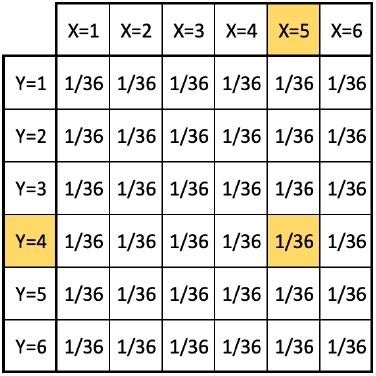
\includegraphics[width=0.5\linewidth]{./img/joint_probability.png} \\
\textbf{Independant random Variables}
\begin{itemize}
    \item Joint Probability is the product of the individual probabilities
\end{itemize}
$P(X,Y) = P(X) * P(Y)$ (only if independant)\\ 
$P(X,Y,Z) = P(X) * P(Y) * P(Z)$ (only if independant)\\
\textbf{Correlated random Variables}
\begin{itemize}
    \item There are events that are not independant
    \item Such random variables are correlated
    \item $X$: observe clouds (0=no, 1=small, 2=big)
    \item $Y$: observe rain (0=no, 1=light, 2=moderate, 3=heavy)
\end{itemize}
\textbf{Conditional Probability}
\begin{itemize}
    \item One variable is no longer random
    \item X is observed, its value is fixed
    \item Calculate the probabilities of Y given X: $P(Y | X)$
\end{itemize}
$P(X, Y) = P(X | Y) * P(Y)$\\ 
$P(X, Y) = P(Y | X) * P(X)$\\
$P(Y | X) = \frac{P(X,Y)}{P(X)}$\\ 
\textbf{Bayes Rule}\\
$P(X|Y)*P(Y) = P(Y|X)*P(X)$\\ 
Therefore:\\
$P(Y|X) = \frac{P(X|Y)*P(Y)}{P(X)}$